\chapter{Evaluation}
\section{Vorgehensweise}
In diesem Kapitel soll der erreichte Grad der Integration des Microblaze in die SpartanMC Entwicklungsumgebung evaluiert werden. Dabei soll nicht nur gezeigt werden, dass auf Microblaze basierende Systeme erstellt und synthetisiert werden können, sodern auch, dass die Integration die ursprüngliche Funktionalität nicht negativ beeinflusst. Hierzu soll zunächst ein einfaches System mit allen hinzugefügten Komponenten mit JConfig erstellt, anschließend mit der Toolchain ein Bitfile erzeugt werden. Außerdem sollen die Aktualisierung des Bitfiles und die Speicherinitialisierung für die Simulation ausgeführt werden. Dies soll zeigen, dass die Integration des Microblaze in JConfig erfolgreich war und dass die Anpassungen an den Makefiles zur Speicherinitialisierung ebenfalls funktionieren.\\
Desweiteren soll Software mit dem SDK von Xilinx geschrieben werden, welche sowohl die FSL-Blöcke als auch den UART-Core verwendet. Mit data2mem soll aus dem entstehenden ELF-File eine Speicherinitialisierung für die Simulation in Form einer Verilog-Datei erfolgen. Das System muss anschließend simuliert werden um die Funktionalität der einzelnen Systemkomponenten zu verifizieren.\\
Um zu zeigen, dass die Änderungen keinen negativen Einfluss auf SpartanMC-Systeme haben, soll der Workflow mit zwei weiteren Systemen durchlaufen werden. Das eine System soll nur SpartanMC-Instanzen beinhalten, während das andere sowohl einen SpartanMC, als auch einen Microblaze beinhalten.
\section{Erstellen des Testsystems mit JConfig}
Das für die Evaluation verwendete System ist in Abbildung \ref{fig:Testsystem} dargestellt. Im Folgenden wird der Aufbau des Systems und das Vorgehen bei der Erstellung kurz beschrieben.
\begin{figure}[th!]
	\centering
	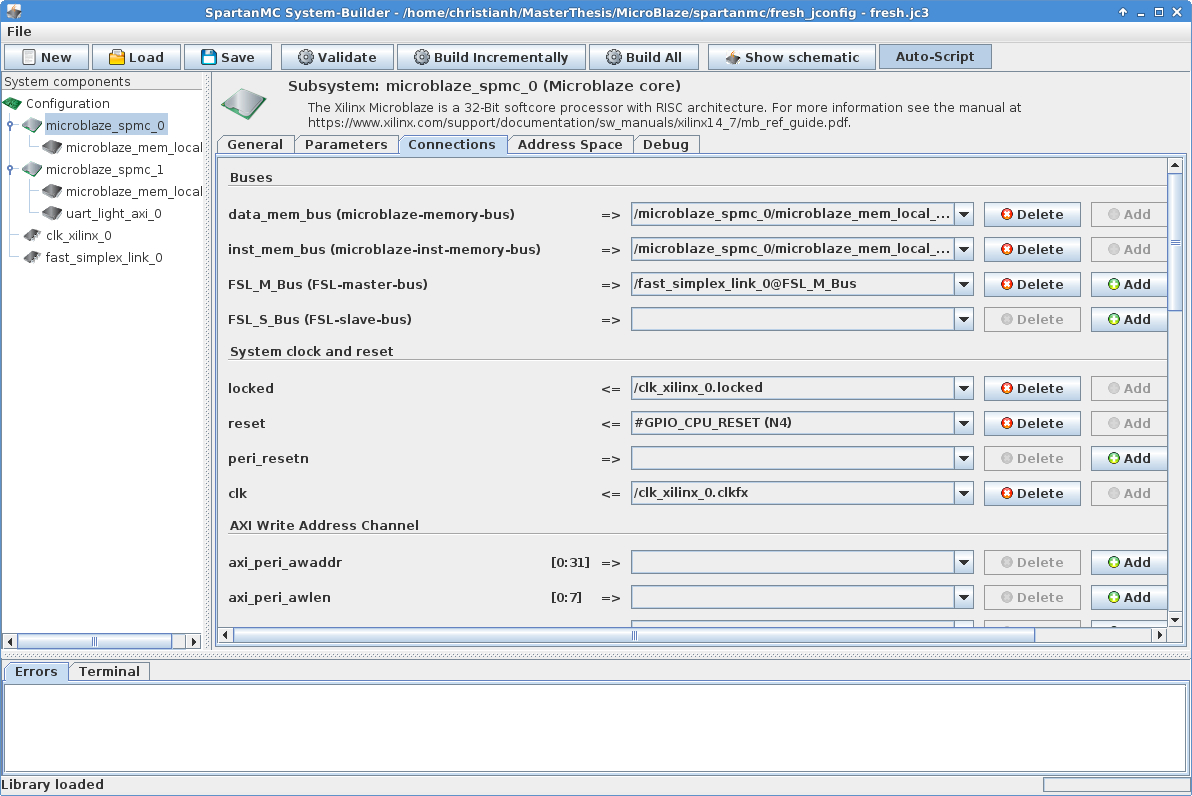
\includegraphics[width=1\linewidth]{./bilder/Testsystem}
	\caption{Testsystem zur Evalutation des erreichten Grades der Integration}
	\label{fig:Testsystem}
\end{figure}
Den Kern des Systems stellen zwei Microblaze dar, deren Parametrisierung sich nur durch das Setzen des Parameters \textit{C\_FSL\_LINKS} auf 1 von der Default-Parametrisierung unterscheidet. Desweiteren verfügen die Prozessoren über 8KByte Speichermodule. Ein UART-Modul ist an den zweiten Microblaze Prozessor angeschlossen und es existiert ein FSL-Core, der eine unidirektionale Verbindung von \textit{microblaze\_spmc\_0} zu \textit{microblaze\_spmc\_1} realisiert. Die Parametrisierungen entsprechen hierbei den Standardeinstellungen. Desweiteren wurde ein Modul zur Takterzeugung hinzugefügt, welches einen Takt von ~49.8MHz erzeugt. Dieser Taktwert wird im Hinblick auf das mit XPS generierte Referenzsystem gewählt, da  dort ein Takt von 50MHz generiert wird und diese Einstellung mit dem Taktmodul aus der SpartanMC Entwicklungsumgebung nicht exakt reproduziert werden kann.\\
Beim Verbinden der einzelnen Module fällt auf, dass das Zusammenfassen der Signale für Speicher und FSL zu Bussen die Arbeit erleichtert und das Interface übersichtlich hält, während das Verbinden der einzelnen AXI-Signale deutlich mehr Aufwand erfordert. Desweiteren ist die Wahrscheinlichkeit ein Signal falsch zu verbinden durch die schiere Anzahl an Signalen relativ hoch.\\
Die Parametrisierung der neuen Module wird durch die Gliederung mehrerer Parameter in logische Gruppen übersichtlich gestalltet. Die Beschreibungen neben den Parametern geben Auskunft über ihre Bedeutung und in der Modulbeschreibung wird auf das Microblaze Handbuch verwiesen, um genauere Informationen zu den Parametern zu erhalten. Durch das Aliasing von einigen Parametern, sind deren Auswahlmöglichkeiten deutlich aussagekräftiger.\\
Im Vergleich zum SpartanMC ist der Grad der Automatisierung noch relativ gering. Für den SpartanMC existiert ein Groovy-Skript, welches automatisch eine Speicherinstanz zum Design hinzufügt und gleichzeitig Verbindungen zum Taktmodul erstellt. Dies wäre für den Microblaze auch denkbar und würde die Inkludierung eines Moduls etwas erleichtern.\\
Zusammenfassend lässt sich sagen, dass das Erstellen von Microblaze-Systemen dem Erstellen von SpartanMC-Systemen sehr ähnelt. Der Grad der Automatisierung lässt sich durch Groovy-Skripte noch erhöhen und der Arbeitsaufwand zum Verbinden der AXI-Signale durch Busbeschreibungen reduzieren. Desweiteren wäre es wünschenswert, dass der Parameter \textit{C\_FSL\_LINKS} des Microblaze automatisch, basierend auf der Anzahl der verwendeten FSL-Interfaces gesetzt wird. Alles in allem lassen sich Microblaze-Systeme in JConfig jedoch einfach und verhältnismäßig schnell ohne die Verwendung von Xilinx-spezifischen grafischen Oberflächen erstellen.
\section{Verwendung der Toolchain} \label{sec:toolChainUsage}
Zum Testen der Toolchain wurden zunächst mit dem Befehl \textit{make newfirmware} ein neues Verzeichnis für eine SpartanMC-Firmware erstellt. Diese Dummy-Firmware soll nur dem Zweck dienen, die Toolchain zu testen und kann nicht verwendet werden, um die Funktionalität der Systemkomponenten in der Simulation zu verifizieren. Bevor durch den Befehl \textit{make all} ein Bitfile generiert wird, wird überprüft, ob die von JConfig generierten Dateien, die durchgeführten Änderungen übernommen haben. Dies umfasst folgende Dateien:
\begin{itemize}
	\item \textbf{configuration.v}: Hier wird überprüft, ob alle Module aus JConfig instanziiert werden und sowohl die Parameter, als auch die Verbidungen korrekt gesetzt werden.
	\item \textbf{firmwares.mk}: In dieser Datei sollte die Liste \textit{JCONFIG\_SPARTANMC\_FIRMWARE\_IDS} leer sein und \textit{JCONFIG\_MICROBLAZE\_FIRMWARE\_IDS} die Namen der beiden Speicherinstanzen beinhalten.
	\item \textbf{project.mk}: Die Konstante \textit{JCONFIG\_SIMULATION\_LIBRARY\_PATH} muss definiert sein und den Pfad zu den Simulationslibraries angeben.
	\item \textbf{sim\_lib.mk}: Hier muss überprüft werden, ob die Liste \textit{JCONFIG\_SIM\_LIBRARIES} alle notwendigen Libraries definiert.
	\item \textbf{spartanmc\_worklib.fdo}: Das Do-Skript darf nur Befehle zur Kompilierung von HDL-Dateien enthalten, die nicht einer der vorkompilierten Libararies angehören.
	\item \textbf{memory.bmm}: Hier muss sichergestellt werden, dass für jeden, mit einem Microblaze verbundenen Speicher, eine \textit{ADDRESS\_MAP} erzeugt wird. Dabei sollte auf Name und Größe des Speichers, sowie die Definitionen der Bitlanes geachtet werden.
	\item \textbf{memory.xml}: Diese Datei darf nicht erstellt werden, da es keinen SpartanMC im SoC gibt.
\end{itemize}
Unter Berücksichtigung der angegebenen Kriterien, wird während der Überprüfung der Dateien festgestelt, dass kein fehlerhaftes Verhalten beobachtet werden kann. Mit \textit{make all} wird nun die Erzeugung des Bitfiles initiiert und es werden alle Schritte von der Synthese bis hin zur Generierung des Bitfiles durchlaufen. Vor dem Schritt Translate werden die ELF-Dateien erzeugt und es können in der Konsole die Aufrufe von data2mem zur Erzeugung der UCF-Dateien beobachtet werden. Ein Blick in die Datei \textit{spartanmc.ucf} zeigt, dass die Initialisierung der Speicherblöcke in der Datei vorhanden ist. Es wird von einer korrekten Erzeugung ausgegangen, da für die Inintialisierung mit data2mem ein, von der Qualitätssicherung von Xilinx freigegebenes Tool verwendet wurde. Desweiteren wird im Abschnitt \ref{sec:simRes} darauf eingegangen, ob gültige Instruktionen während der Simulation aus dem Speicher gelesen werden können. Aus den Berichten für die einzelnen Schritte der Erzeugung des Bitfiles (von Synthese bis hin zu Place-and-Route) kann außerdem herausgelesen werden, dass tatsächlich Hardware generiert wurde.\\
Die Aktualisierung des Bitfiles wird mit dem Befehl \textit{make bitgen} getestet. Beim Aufruf werden in der Konsole die einzelnen Aufrufe von data2mem dargestellt.\\
Um die Anpassungen an der Toolchain für die Simulation zu testen, wird mit dem Befehl \textit{make newsim} ein neues Verzeichnis für die Simulation angelegt. In diesem Verzeichnis befindet sich unter anderem die Testbench, ein Do-Skript, welches die Simulation steuert und ein eine Intialisierungsdatei für Modelsim, welche die Library-Mappings enthält. Durch Eingabe des Befehls \textit{vsim -do testbench.fdo} wird der Simulator gestartet und das Do-Skript ausgeführt. Während der Ausführung des Skripts wird die Datei \textit{modelsim.ini} dahingehend erweitert, das sie die Mappings der Xilinx Simulationslibraries enthält. Modelsim kompiliert alle relevanten Dateien und kann dann verwendet werden. Fehlermeldungen treten nicht auf. Die Speicherinitialisierung für die Simualtion ist in der Datei \textit{spartanmc\_sim.v} zu finden und wird ebenfalls korrekt erstellt.
\section{Erstellen der Testsoftware und Erzeugung der Speicherinitialisierung für die Simulation}
Da der Microblaze GCC noch nicht in die SpartanMC Toolchain integriert ist, muss die Software mittels Xilinx SDK erstellt werden. Hierzu wird zunächst mit XPS das System in Abbildung \ref{fig:XPS_ReferenceSystem} erzeugt. Die Konfiguration des Systems entspricht größtenteils der, des von JConfig erzeugten Systems. Einzige Unterschiede sind, dass in XPS der AXI-Bus verwendet werden muss und das Modul zur Takterzeugung ein anderes ist. Es wird ein Takt von 50Mhz erzeugt. Anschließend werden Netzliste und Bitfile generiert und das Design zum SDK exportiert.

\begin{figure}[th!]
	\centering
	\includegraphics[width=1\linewidth]{./bilder/XPS_ReferenceSystem}
	\caption{}
	\label{fig:XPS_ReferenceSystem}
\end{figure}
\noindent
Im SDK werden zunächst über \textit{``New --> Application Project''} für jeden der beiden Prozessoren neue \textit{``Hello World''}-Projekte und BSP angelegt. Nun wird folgende Applikation implementiert. Ein Prozessor sendet über das FSL-Interface den String \textit{``Hello World!''} an den anderen Prozessor, welcher wiederum den empfangenen String über die UART verschickt. Mit dieser simplen Applikation werden alle, in die SpartanMC Entwicklungsumgebung integrierten Komponenten verwendet. Der Code für beide Prozessoren ist nachfolgend aufgeführt.
\begin{lstlisting}
/**Code for the sending processor*/
#include <stdio.h>
#include "platform.h"
#include <fsl.h>
#include <xparameters.h>

void print(char *str);

int main()
{
	int i = 0;
    init_platform();

    char* string = "Hello World!\n\r";
    while(1){
    	for (i=0;i<13;i++){
			putfslx(string[i],0,FSL_NONBLOCKING);
		}
    }
    return 0;
}
\end{lstlisting}
\begin{lstlisting}
/**Code for the receiving processor*/
#include <stdio.h>
#include "platform.h"
#include <fsl.h>

void print(char *str);

int main()
{
	int i = 0;
    init_platform();

    char* string = "";
    while(1){
		for (i=0;i<13;i++){
			getfslx(string[i],0,FSL_DEFAULT);
		}
		print(string);
    }
    return 0;
}
\end{lstlisting}
\noindent
Die verwendeten Macros \textit{putfslx} und \textit{getfslx} sind in der Header-Datei \textit{fsl.h} mittels Inline-Assembler definiert. Weitere allgemeine Informationen zu Treibern können in dem Dokument \textit{OS and Libraries Document Collection} \cite{OSLIB} gefunden werden. Das SDK erzeugt aus dem Code automatisch zwei ELF-Dateien. Mit diesen ELF-Dateien kann nun manuell der Speicher des Microblaze in der SpartanMC Entwicklungsumgebung initialisiert werden. Hierzu werden mittels data2mem zwei Verilog-Dateien aus den beiden ELF-Dateien und der \textit{memory.bmm} erzeugt. Mit dem Skript \textit{mksim} im Verzeichnis \textit{``spartanmc/hardware/microblaze/example''} können die beiden Dateien zusammengeführt werden. Der Name der neuen Datei ist \textit{init\_ram.v}. Diese Speicherintialisierung wird im Verzeichnis \textit{build} des SpartanMC-Projekts abgelegt. Nun muss nur noch in der Datei \textit{spartanmc\_worklib.fdo} der Eintrag für \textit{spartanmc\_sim.v} zu \textit{init\_ram.v} geändert werden. Mit diesen Anpassungen ist das System nun bereit für die Simulation.

\section{Simulationsergebnisse}\label{sec:simRes}
\subsection{Lesen von Instruktionen aus dem Speicher}
In der Simulation soll zunächst gezeigt werden, dass Instruktionen erfolgreich aus dem Speicher gelesen werden. Abbildung \ref{fig:InstFetch} zeigt, wie Instruktionen in den Instruction-Buffer des Microblaze gelesen werden. Als Referenz, welche Werte zu erwarten sind, ist in Abbildung \ref{fig:ELF_Snap} ein Auschschnitt aus der ELF-Datei dargestellt.

\begin{figure}[th!]
\centering
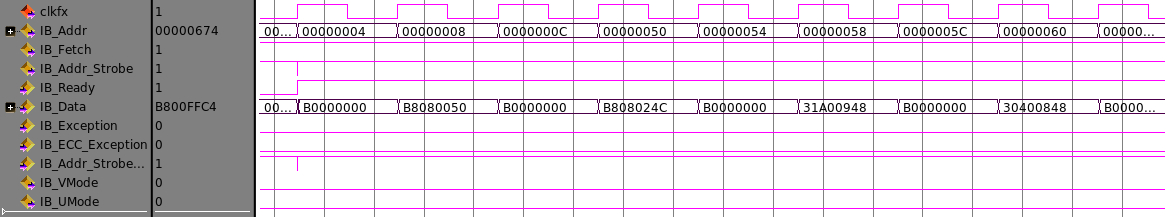
\includegraphics[width=1\linewidth]{./bilder/InstFetch}
\caption{Simulation des Instruction-Buffers des Microblaze}
\label{fig:InstFetch}
\end{figure}
\begin{figure}[th!]
\centering
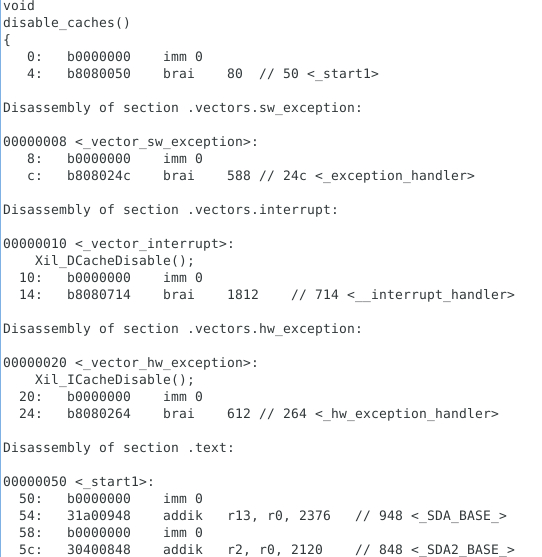
\includegraphics[width=0.7\linewidth]{./bilder/ELF_Snap}
\caption{Ausschnitt aus der ELF-Datei des sendenden Microblaze}
\label{fig:ELF_Snap}
\end{figure}
\noindent
Es lässt sich feststellen, dass sich die Einträge aus der ELF-Datei in der Simulation des Instruction-Buffers wiederfinden lassen. So kann davon ausgegangen werden, dass der Zugriff auf den Speicher funktioniert.
\subsection{Kommunikation über das FSL-Interface}
Als nächstes wird gezeigt, wie Daten über das FSL-Interface gesendet und aus dem FSL-Block gelesen werden. Hierzu wird Abbildung \ref{fig:FSL_SIM} betrachtet.
\begin{figure}[th!]
\centering
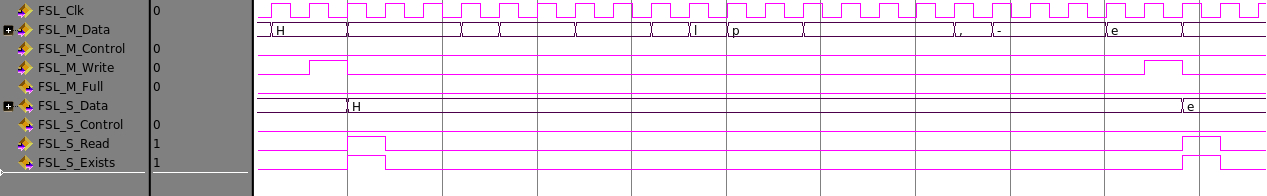
\includegraphics[width=1\linewidth]{./bilder/FSL_SIM}
\caption{Simulation des FSL-Moduls}
\label{fig:FSL_SIM}
\end{figure}
Es kann beobachtet werden, wie das \textit{'H'} des String \textit{``Hello World!''} übertragen wird. Hierzu wird das Signal \textit{FSL\_M\_WRITE} vom Master gesetzt, sodass im nächsten Takt das Signal \textit{FSL\_S\_EXISTS} dem Slave signalisiert, dass Daten im FIFO-Speicher vorhanden sind. Der Slave reagiert mit dem Setzen von \textit{FSL\_S\_READ}, um die Daten zu lesen. Basierend auf den Simulationsergebnissen kann angenommen werden, dass der FSL-IP-Core funktioniert.
\subsection{Versenden von Daten über den UART-Core}
Die Simulation des UART-Cores ist in Abbildung \ref{fig:UART_SIM} dargestellt.
\begin{figure}[th!]
\centering
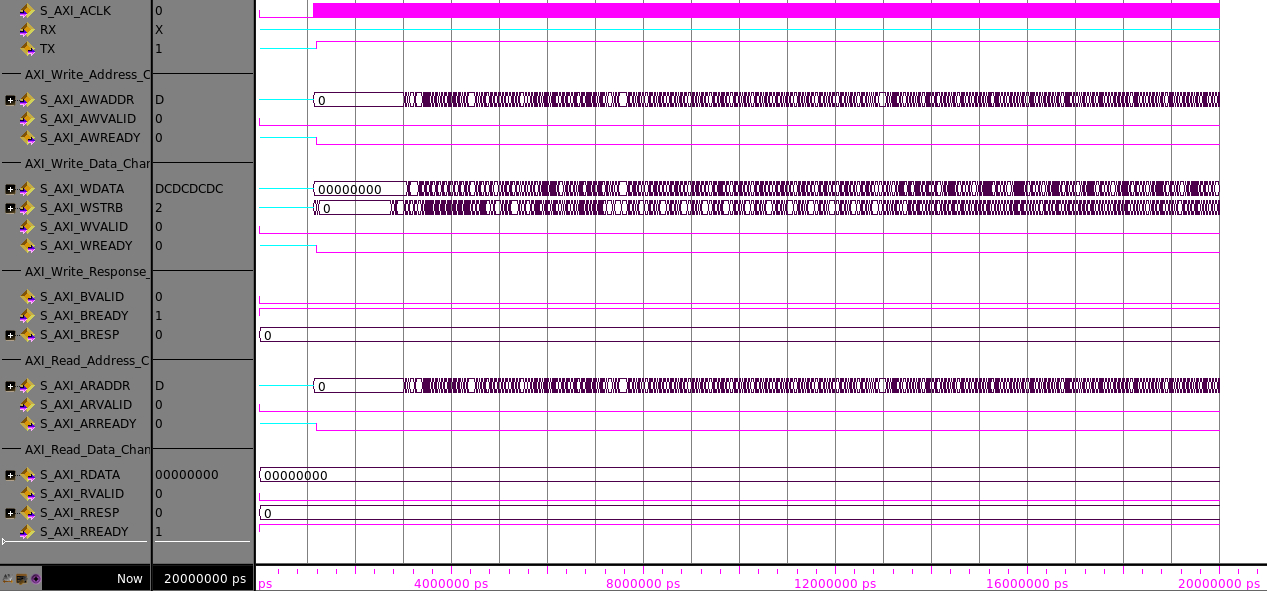
\includegraphics[width=1\linewidth]{./bilder/UART_SIM}
\caption{Simulation des UART-Cores}
\label{fig:UART_SIM}
\end{figure}
Über einen Verlauf von 20\textmu/s kann beobachtet werden, dass die Valid- und Ready-Signale der einzelnen Kanäle konstant sind. Somit findet keine Übertragung statt. Als Vergleich wird das mit XPS generierte System simuliert, um zu prüfen, ob die selben Probleme auch im Referenzsystem auftauchen. Hierzu wird die Project-Datei des Referenzsystems in ISE importiert und eine Testbench erzeugt. Mit dem Xilinx Simulator ISIM wird die Simulation gestartet. Die Ergebnisse sind in Abbildung \ref{fig:UART_ISIM} dargestellt.
\begin{figure}[th!]
\centering
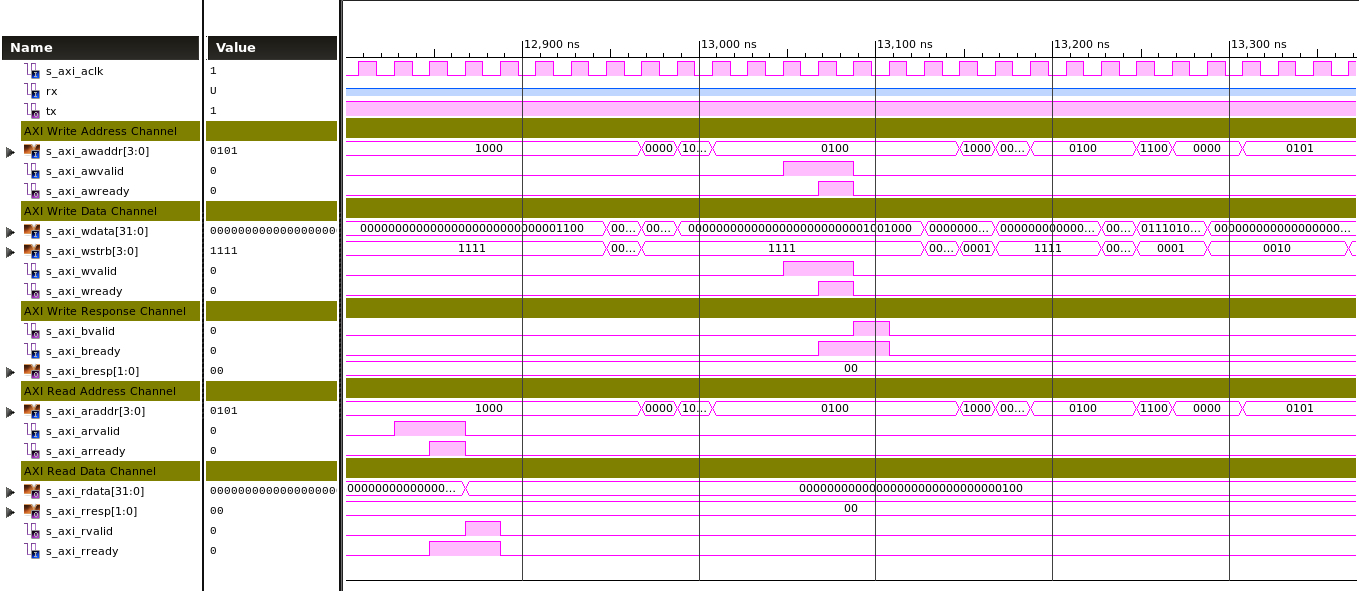
\includegraphics[width=1\linewidth]{./bilder/UART_ISIM}
\caption{Simulation des UART-Cores im Referenzsystem mit ISIM}
\label{fig:UART_ISIM}
\end{figure}
Wie man sehen kann, wird nach ca. 12.8\textmu/s im Read Address Channel das Steuersignal \textit{s\_axi\_arvalid} gesetzt. Auf Seiten des Microblaze, ist dieses Verhalten ebenfalls zu beobachten (es wird der Übersicht halber in der Abbildung nicht dargestellt). Die Kommunikation über den AXI-Bus wird fortgesetzt und nach ca. 90\textmu/s kann beobachtet werden, wie das TX-Signal des UART-Cores sich verändert.\\
Der Grund für dieses Verhalten des Microblaze in der SpartanMC Entwicklungsumgebung konnte aus zeitliche Gründen im Rahmen dieser Arbeit nicht mehr ermittelt werden. Die Unterschiede zwischen den beiden Systemen sind der AXI-Busses und die Takterzeugung. In der Simulation mit ISIM kann allerdings beobachtet werden, dass sämtliche Eingangssignale des AXI-Interfaces des Microblaze sich vor dem Setzen des \textit{s\_axi\_arvalid}-Signals nicht verändern. Der Microblaze startet die Übertragung also von sich aus, was bedeutet, dass der fehlende AXI-Bus in der SpartanMC Umgebung nicht das Problem sein kann. Die Ursache des Problems muss daher beim Microblaze liegen. Eine Vergleich mit der Parameterisierung des Microblaze im Referenzsystem hat allerdings keine Erkenntnis über die Ursache des Verhaltens gebracht.
\section{SpartanMC- und Hybrid-Systeme}
Da keine Veränderung am SpartanMC vorgenommen wurden, werden lediglich die gleichen Tests, wie in Abschnitt \ref{sec:toolChainUsage} durchgeführt. Das erste Testsystem besteht aus zwei SpartanMC und das zweite System aus je einem SpartanMC und Microblaze. Desweiteren werden zusätzlich UART-Module als Peripherie hinzugefügt, um zu verhindern, dass Hardware während der Synthese wegoptimiert wird.\\
Für das erste System terminieren die Tests ohne Fehler. Die UCF-Datei mit der Speicherinitialisierung wird korrekt erzeugt und auch der Aufruf von \textit{make bitgen} aktualisiert die Bitfiles entsprechend. Desweiteren lässt sich das System auch wie gewohnt simulieren. Es sei noch anzumerken, dass im Falle eines reinen SpartanMC-Systems die Datei \textit{memory.bmm} nicht generiert wird.\\
Die Tests für das zweite System haben gezeigt, dass die Toolchain Hybrid-Systeme handhaben kann. Sowohl die Speicherinitialisierung per UCF-Datei, als auch die Aktualisierung des Bitfiles, durch ausführen von \textit{make bitgen}, laufen erfolgreich durch. Die Simulation startet ebenfalls ohne Fehlermeldungen und die Verilog-Datei \textit{spartanmc\_sim.v} wird korrekt erzeugt. 